Die deflektometrische Registrierung \acrshort{lr} kann nicht ohne Weiteres direkt ausgewertet werden.
Deshalb wird im Folgenden die Weiterverarbeitung der deflektometrischen Registrierung beschrieben, sodass bekannte Methoden aus dem Gebiet der Bildverarbeitung angewendet werden können.

\p
Die graphische Darstellung der deflektometrischen Registrierung \acrshort{lr} stellt sich zunächst als schwierig heraus, da man mit einer Abbildung der Form $\mathbb{R}^2 \rightarrow \mathbb{R}^2$ arbeitet.
Aus dem Grund wird die Separierbarkeit der deflektometrischen Registrierung aus Satz \ref{theo:separierbarkeitDeflektometrischeRegistrierung} angewendet.
Daraus erhält man die beiden Abbildungen der Form $\mathbb{R}^2 \rightarrow \mathbb{R}$:
%
\begin{equation*}
	\acrshortmath{lrx} : \mathbb{R}^{2} \supset A_{Cam} \rightarrow \mathbb{R} ,\quad (x_{B}, y_{B}) \mapsto x_{L}
\end{equation*}
%
\begin{equation*}
	\acrshortmath{lry} : \mathbb{R}^{2} \supset A_{Cam} \rightarrow \mathbb{R} ,\quad (x_{B}, y_{B}) \mapsto y_{L}
\end{equation*}
%
In der Form lässt sich die Analogie zu der mathematischen Beschreibung eines Graubildes $f$ erkennen:
%
\begin{equation*}
	f : \mathbb{R}^{2} \supseteq [x_{min},x_{max}] \times [y_{min},y_{max}] \rightarrow [I_{min},I_{max}] \subseteq \mathbb{R} ,\quad (x,y) \mapsto f(x,y)
\end{equation*}
%
Für die Darstellung als Bilder sind somit lediglich geeignete Transformationen der Wertemengen der deflektometrischen Registrierungen \acrshort{lrx} und \acrshort{lry} nötig.
%
\begin{Definition}{Darstellung der Deflektometrischen Registrierung}{def:graphDeflektometrischeRegistrierung}
	Die deflektometrischen Registrierung \acrshort{lr} kann als zwei einzelne Graubilder \acrshort{frx} und \acrshort{fry} dargestellt werden.
	%	
	\begin{equation*}
		\acrshortmath{frx} : \mathbb{R}^2 \supset \acrshortmath{d}(\acrshortmath{lrx}) \rightarrow [I_{min},I_{max}] \subseteq \mathbb{R}
	\end{equation*}
	%
	\begin{equation*}
		\acrshortmath{fry} : \mathbb{R}^2 \supset \acrshortmath{d}(\acrshortmath{lry}) \rightarrow [I_{min},I_{max}] \subseteq \mathbb{R}
	\end{equation*}
	%
	Dabei lassen sich die Bilder \acrshort{frx} und \acrshort{fry} schreiben als:
	%	
	\begin{equation*}
		\acrshortmath{frx}(x,y) = t_x(\acrshortmath{lrx}(x,y))
	\end{equation*}
	%	
	\begin{equation*}
		\acrshortmath{fry}(x,y) = t_y(\acrshortmath{lry}(x,y))
	\end{equation*}
	%
	Es gilt $\acrshortmath{d}(\acrshortmath{frx}) = \acrshortmath{d}(\acrshortmath{lrx})$ und $\acrshortmath{d}(\acrshortmath{fry}) = \acrshortmath{d}(\acrshortmath{lry})$.
	Die Abbildungen $t_x$ und $t_y$ sind dabei lineare Transformationen der Wertemengen der deflektometrischen Abbildungen in Spalten und Zeilen zu den zulässigen Intensitäten für die Bilder \acrshort{frx} und \acrshort{fry}, angegeben durch das Intervall $[I_{min},I_{max}]$.
	%
	\begin{equation*}
		t_x : \mathbb{R} \supset \acrshortmath{w}(\acrshortmath{lry}) \rightarrow [I_{min},I_{max}] \subseteq \mathbb{R}
	\end{equation*}
	%
	\begin{equation*}
		t_y : \mathbb{R} \supset \acrshortmath{w}(\acrshortmath{lry}) \rightarrow [I_{min},I_{max}] \subseteq \mathbb{R}
	\end{equation*}
	%
	Die Transformationen $t_x$ und $t_y$ lassen sich schreiben als:
	%	
	\begin{equation*}
		t_x(x) = \left(\dfrac{x}{\acrshortmath{lwidth}}(I_{max} - I_{min})\right) + I_{min}
	\end{equation*}
	%	
	\begin{equation*}
		t_y(y) = \left(\dfrac{y}{\acrshortmath{lheight}}(I_{max} - I_{min})\right) + I_{min}
	\end{equation*}
	%
\end{Definition}
%
Erstellt man aus der berechneten deflektometrischen Registrierung \acrshort{lr} einer ungekrümmten Fläche die zugehörigen Bilder \acrshort{frx} und \acrshort{fry} nach Definition \ref{def:graphDeflektometrischeRegistrierung}, erhält man Darstellungen wie in Abbildung \ref{tikz:abbOptimaleSpaltenZeilenReg}:

% Abbildung: Optimale Spalten- und Zeilenregistrierung
{
	\begin{figure}[H]
		\centering
		\begin{adjustbox}{width=\textwidth}
	\begin{tikzpicture}[every node/.style={inner sep=0,outer sep=0}]
	
		\node [anchor=north west] (imgSpalten) at (0,0) {
\includegraphics[width=.47\textwidth]{04_deflektometrischeRegistrierung/auswertungDeflektometrischeRegistrierung/figures/spaltenRegistrierung_optimal}};
		\node [below=0.2cm of imgSpalten] {Graubild der Spaltenzuordnung \acrshort{frx}$(x,y)$};
		\node [anchor=north west] (imgZeilen) at (0.53\textwidth,0) {
\includegraphics[width=.47\textwidth]{04_deflektometrischeRegistrierung/auswertungDeflektometrischeRegistrierung/figures/zeilenRegistrierung_optimal}};
		\node [below=0.2cm of imgZeilen] {Graubild der Zeilenzuordnung \acrshort{fry}$(x,y)$};
	
	\end{tikzpicture}
\end{adjustbox}
\caption[Darstellung Spalten- und Zeilenregistrierung]{Darstellung der Spalten- und Zeilenregistrierung als Bilder in Graustufen mit $I_{min} = 0$ und $I_{max} = 255$. Je dunkler ein Pixel ist, desto weiter links bzw. oben befindet sich die zugeordnete Spalten- bzw. Zeilenposition.}
		\label{tikz:abbOptimaleSpaltenZeilenReg}
	\end{figure}
}

\noindent
In Abbildung \ref{tikz:abbOptimaleSpaltenZeilenReg} wird direkt das Muster auf dem Monitor betrachtet.
Aus dem Grund lässt sich erkennen, dass die Zuordnung von Monitor- und Kamerapixeln in den Spalten und Zeilen linear verläuft.
Werden nun die Streifen durch besondere Oberflächeneigenschaften gekrümmt oder verzerrt, dann werden an diesen Stellen in den Bildern der deflektometrischen Registrierung Abweichungen vom linearen Grauwerteverlauf sichtbar.

% Abbildung: Brillenglas Registrierung
{
	\begin{figure}[H]
		\centering
		\begin{adjustbox}{width=\textwidth}
	\begin{tikzpicture}[every node/.style={inner sep=0,outer sep=0}]
	
		\node [anchor=north west] (imgSpalten) at (0,0) {\includegraphics[width=.47\textwidth]{04_deflektometrischeRegistrierung/auswertungDeflektometrischeRegistrierung/figures/streifenKrümmung_spalten}};
		\node [below=0.2cm of imgSpalten] {Graubild der Spaltenzuordnung \acrshort{frx}$(x,y)$};
		\node [anchor=north west] (imgZeilen) at (0.53\textwidth,0) {\includegraphics[width=.47\textwidth]{04_deflektometrischeRegistrierung/auswertungDeflektometrischeRegistrierung/figures/streifenKrümmung_zeilen}};
		\node [below=0.2cm of imgZeilen] {Graubild der Zeilenzuordnung \acrshort{fry}$(x,y)$};
	
	\end{tikzpicture}
\end{adjustbox}
\caption[Darstellung verzerrter Spalten- und Zeilenregistrierung]{Darstellung verzerrter Spalten- und Zeilenregistrierung als Bilder. Verzerrungen entstehen durch tiefe Eingravierungen im Glas.}
		\label{tikz:abbBrillenglasRegistrierung}
	\end{figure}
}

\noindent
Die deflektometrische Registrierung macht bestimmte Fehlstellen in Abbildung \ref{tikz:abbBrillenglasRegistrierung} kenntlich.
Diese Fehlstellen sind allerdings nur tiefe Eingravierungen, durch welche die Phase des Streifenmusters lokal deformiert wird.
Normale Kratzer beeinflussen besonders den durch die Kamera gemessenen Grauwert.
Die zugeordnete Monitorposition hingegen wird durch solche Kratzer nur geringfügig verändert, weshalb diese im Bild der deflektometrischen Registrierung kaum erkennbar sind.
Besser funktioniert die Fehlstellenerkennung, indem man die Reflexionen bzw. die Spiegelbilder der Muster aufnimmt.
So ist es möglich, wie in Abbildung \ref{tikz:abbRegistrierungDelle}, z. B. Dellen und Beulen auf spiegelnden Oberflächen durch die deflektometrische Registrierung deutlich hervorzuheben.

% Abbildung: Objekt mit Delle
{
	\begin{figure}[H]
		\centering
		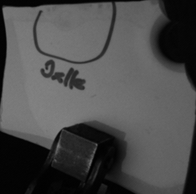
\includegraphics[width = 0.47\textwidth]{04_deflektometrischeRegistrierung/auswertungDeflektometrischeRegistrierung/figures/delleBeleuchtet}
		\caption[Spiegelndes Porzellanbruchstück mit Delle]{Spiegelndes Porzellanbruchstück mit Delle.}
		\label{img:objektMitDelle}
	\end{figure}
}

% Abbildung: Deflektometrische Registrierung bei Objekt mit Delle
{
	\begin{figure}[H]
		\centering
		\begin{adjustbox}{width=\textwidth}
	\begin{tikzpicture}[every node/.style={inner sep=0,outer sep=0}]
	
		\node [anchor=north east] (imgSpalten) at (-0.03\textwidth,0) {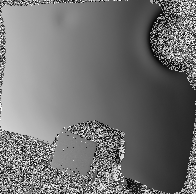
\includegraphics[width=.47\textwidth]{04_deflektometrischeRegistrierung/auswertungDeflektometrischeRegistrierung/figures/spaltenRegistrierung_Delle}};
		\node [below=0.2cm of imgSpalten] {Graubild der Spaltenzuordnung \acrshort{frx}$(x,y)$};
		\node [anchor=north west] (imgZeilen) at (0.03\textwidth,0) {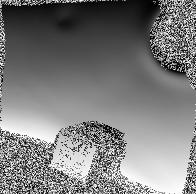
\includegraphics[width=.47\textwidth]{04_deflektometrischeRegistrierung/auswertungDeflektometrischeRegistrierung/figures/zeilenRegistrierung_Delle}};
		\node [below=0.2cm of imgZeilen] {Graubild der Zeilenzuordnung \acrshort{fry}$(x,y)$};
		
	\end{tikzpicture}
\end{adjustbox}
\caption[Deflektometrische Registrierung bei Delle]{Deflektometrische Registrierung des spiegelnden Keramikobjekts aus Abbildung \ref{img:objektMitDelle}.}
		\label{tikz:abbRegistrierungDelle}
	\end{figure}
}

\noindent
In Abbildung \ref{tikz:abbRegistrierungDelle} entsteht im Hintergrund um das Objekt herum eine Störumgebung.
Der Grund dafür ist die fehlende Reflexion des Musters und somit ähnliche Grauwerte in den phasenverschobenen Bildern.
Dies führt dazu, dass in der Bestimmung der Phase $\phi$ für solche Pixel numerisch instabile Ausdrücke und somit schwankende Werte vorkommen.

\p
Die resultierenden Bilder können durch herkömmliche Verfahren aus der Bildverarbeitung weiterverarbeitet und analysiert werden.
Durch die weichen Grauwertverläufe an gleichmäßig gekrümmten Oberflächen in den \acrshort{frx} und \acrshort{fry}, lassen sich diese Bilder effizient über ihre Gradienten analysieren (siehe Abbildung \ref{tikz:abbGradientenbildReg}).
Abrupte Änderungen der Grauwerte innerhalb des spiegelnden Objekts führen zu höheren Gradienten als in der Umgebung. Fehlstellen wie z. B. Dellen oder Pickel lassen sich damit gut detektieren.
Aus demselben Grund erweisen sich auch Hochpassfilterungen als hilfreich \cite{kit_werling}.

% Abbildung: Gradientenbild der deflektometrischen Registrierung.
{
	\begin{figure}[H]
		\centering
		\begin{adjustbox}{width=\textwidth}
	\begin{tikzpicture}[every node/.style={inner sep=0,outer sep=0}]
	
		\node [anchor=north east] (imgSpalten) at (-0.03\textwidth,0) {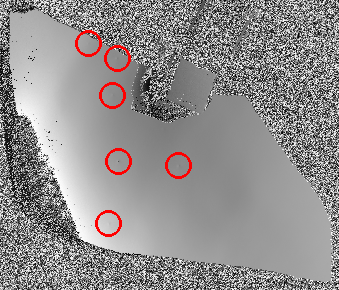
\includegraphics[width=.47\textwidth]{04_deflektometrischeRegistrierung/auswertungDeflektometrischeRegistrierung/figures/pickelDeflektometrischeRegistrierung}};
		\node [below=0.2cm of imgSpalten] {Graubild der Spaltenzuordnung \acrshort{frx}$(x,y)$};
		\node [anchor=north west] (imgGradienten) at (0.03\textwidth,0) {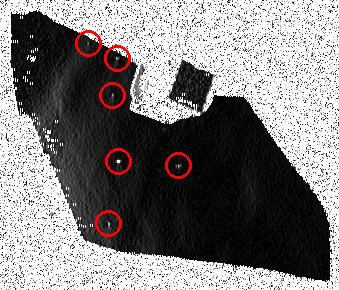
\includegraphics[width=.47\textwidth]{04_deflektometrischeRegistrierung/auswertungDeflektometrischeRegistrierung/figures/pickelGradientenbild}};
		\node [below=0.2cm of imgGradienten, align = center] {Bild der Ableitung von \acrshort{frx}$(x,y)$ \\ in $x$-Richtung};
		
	\end{tikzpicture}
\end{adjustbox}
\caption[Hervorhebung von Pickeln auf reflektierenden Oberflächen.]{Deflektometrische Spaltenregistrierung eines spiegelnden Porzellanbruch\-stücks und das zugehörige Bild der Ableitung. In den rot markierten Stellen lassen sich kleine Abweichungen von einem stetigen Grauwertverlauf erkennen, die in der Ableitung einen Ausschlag haben. Auf dem Prüfobjekt befinden sich an den Stellen kleine Pickel auf der Oberfläche.}
		\label{tikz:abbGradientenbildReg}
	\end{figure}
}

\noindent
Das untersuchte Objekt aus Abbildung \ref{tikz:abbGradientenbildReg} weist am linken Rand vereinzelt matte Stellen auf.
Dadurch treten im Bild der deflektometrischen Registrierung \acrshort{frx} einzelne dunkle Punkte bzw. Artefakte am linken Rand auf.
Diese erkennt man somit auch im Gradientenbild von \acrshort{frx} als Fehlstellen.

\p
In dem Gradientenbild in $x$-Richtung aus Abbildung \ref{tikz:abbGradientenbildReg} lassen sich Aussagen über die Krümmung der Oberfläche entlang der $x$-Richtung treffen.
Allgemein betrachtet man zu\-nächst eine feste Gerade in der Kameraebene, bezeichnet als Bildkurve.
Die Bildkurve entsteht durch die Spiegelung einer bestimmten Monitorkurve auf einer Oberfläche.
Von der Kurve in der Monitorebene schneiden die ausgehenden Lichtstrahlen die Oberfläche entlang einer Oberflächenkurve.
Über den Zusammenhang der Spiegelabbildung von Geraden und Kurven an gekrümmten Oberflächen lässt sich zeigen, dass die Änderung der Monitorkurve vom linearen Verlauf proportional zur Änderung der Flächennormalen entlang der Oberflächenkurve ist \cite{kit_werling}.
Deutlich wird dies nochmals, wenn man beachtet, dass Geraden bei der Spiegelung nur auf Geraden abgebildet werden können, wenn die Spiegeloberfläche an den Reflexionspunkten einer Ebene entspricht.
Das heißt, dass lokale Änderungen der Tangenten an der Monitorkurve lokalen Abweichungen der Spiegeloberfläche vom ebenen Verlauf entsprechen.
Bekanntlich stellt die deflektometrische Registrierung \acrshort{lr} den Zusammenhang zwischen der Bildebene und der Monitorebene dar.
Demzufolge lässt sich durch das Ableiten der deflektometrischen Registrierung \acrshort{lr} in eine bestimmte Richtung direkt die Abweichung der Flächennormalen, also die wahrgenommene Krümmung der Oberfläche, entlang der Richtung bestimmen.
Die wahrgenommene Krümmung steht in direktem Zusammenhang mit der zweiten Ableitung der Objektoberfläche \cite{kit_werling}.

\p
In Abbildung \ref{tikz:abbGradientenbildReg} erhält man durch die Faltung des Bildes \acrshort{frx} mit dem Sobel-Operator für die $x$-Richtung ein Bild, das in direkter Beziehung zu der Ableitung der deflektometrischen Registrierung \acrshort{lr} in  $x$-Richtung steht.
Somit steht dieses Bild auch im Verhältnis mit der Krümmung der Oberfläche in $x$-Richtung.
Analog lässt sich auch die Krümmung in $y$-Richtung auswerten.

\p
Die deflektometrische Registrierung hat im Vergleich zur Rekonstruktion der Oberfläche essenzielle Vorteile.
Zum Einen kann zur Oberflächenprüfung auf die aufwendige Systemkalibrierung verzichtet werden.
Außerdem ermöglichen die Separierbarkeit und die Darstellung als Bilder den Einsatz von effizienten Methoden aus dem Bereich der Bildverarbeitung.
Das ermöglicht den Einsatz dieser Verfahren für die Erkennung von verschiedenen Fehlstellen auf spiegelnden Oberflächen.
Die Verwendung für transparente Objekte, die Licht durchlassen, ist nur eingeschränkt möglich, da die meiste Information in der Krümmung der Streifenmuster liegt.
Nutzt man also den Monitor als Durchlichtbeleuchtung, ist die Zuordnung trotz vorhandener Fehlstellen überwiegend linear.
Dies kann allerdings auch zum Vorteil genutzt werden, wenn nur diese speziellen Informationen gesucht werden.